\section{Simplex Category and Simplicial Sets}

\subsection{Definition of Simplical Sets}

The goal of this mini-project to to define $\infty$-categories via simplicial sets. 
The definition of simplicial sets is based on the \emph{simplex category}, $\D$.

\begin{definition}[Simplex Category \cite{lurie}]
	The \emph{simplex category}, denoted as $\D$, is defined as
	\begin{enumerate}
		\item Its objects linearly ordered finite sets $[n] = \{0 < 1 < \cdots < n\}$ for all $n \geq 0$.
	\item Its morphisms are given by order-preserving maps.
	\end{enumerate}
	Simplex category is also known as the category of combinatorial simplices
\end{definition}

It is clear that $\D$ is equivalent to the category of all finite non-empty totally ordered sets with order-preserving maps. 

For each $n, j \in \N, 0\leq j \leq n$, define \emph{face} and \emph{degenerate} maps repectively as $\D$, $d^{j,n}: [n - 1] \to [n]$ and $s^{j, n}: [n + 1] \to [n]$ given by
\begin{equation}
	d^{j, n}(i) = \begin{cases}
		i & i < j \\
		i + 1 & i \geq j
	\end{cases}, \quad
	s^{j,n}(i) = \begin{cases}
		i & i \leq j \\
		i - 1 & i > j
	\end{cases}.
\end{equation}

Concretely, the face map $d^{j, n}$ is the only injective and order-preserving maps from $[n - 1]$ to $[n]$ that misses $j \in [n]$, and the degenerate map $s^{j, n}$ is the only surjective and order-preserving map from $[n + 1]$ to $[n]$ that hits $j \in [n]$ twice.

Since the domain and codomain of the face and degenerate maps will always be clear from the context, we will drop the superscripts and denote them as $d^j$ and $s^j$.

Let $i < j$. 
The composition of face maps $d^jd^i$ is the unique injective and order-preserving map from $[n - 2]$ to $[n]$ that misses both $i$ and $j \in [n]$. 
A moment of thought shows that this map is the same as $d^id^{j - 1}$.
There are similar relations for the compositions of degenerate maps and mixed compositions of face and degenerate maps. 
All of the identities are listed below.

% TODO: check the middle case
\begin{align}
	d^jd^i &= d^id^{j - 1}, \quad i < j \label{sim1} \\
	s^js^i &= s^is^{j + 1}, \quad i \leq j  \label{sim2} \\
	s^j d^i &= \begin{cases}
		d^i s^{j - 1} & j < i \\
		\text{id} & j = i, i + 1 \\
		d^{i - 1} s^j & j > i + 1
	\end{cases} \label{sim3}
\end{align}

It can be shown that all morphisms in $\D$ can be generated by compositions of face and degenerate maps.

We are now ready to define simplicial sets.

\begin{definition}[Simplicial Set \cite{lurie}]
	A \emph{simplicial set} is presheaf on $\D$, i.e.,
	a functor $X: \D\op \to \S$. 
	We will denote the category of simplicial sets as $\sS$.
\end{definition}

Let $X$ be a simplicial set.
Define $X_n := X([n])$.
We shall define the face map $d_j: X_n \rightarrow X_{n-1}$ as the map induced by the face map on $\D$, $d^j: [n - 1] \to [n]$. 
That is $d_j = Xd^j$. 
Similarly, denote $s_j: X_n \to X_{n + 1}$ the map induced by the degenerate map $s^j: [n + 1] \to [n]$, i.e., $s_j = Xs^j$.
Since $X$ is contravariant, $d_j$ and $s_j$ will satify the following identities, reversing the order of composition compared to \eqref{sim1}, \eqref{sim2}, and \eqref{sim3}. 

\begin{align}
	d_i d_j &= d_{j - 1} d_i, \quad i < j \label{simp1} \\
	d_i s_j &= \begin{cases}
		s_{j - 1} d_{i} & j < i \\
		\text{id} & j = i, i + 1 \\
		s_{j} d_{i - 1} & j > i + 1
	\end{cases} \label{simp3} \\
	s_i s_j &= s_{j + 1} s_i, \quad i \leq j  \label{simp2} 
\end{align}

Since $d^j$ and $s^j$ generates all morphisms in $\D$, the morphisms $d_j$ and $s_j$ will generate all relevant morphisms in $\S$ relevant to $X$ (Recall $X \in [\D\op, \S]$). 
This gives a crucial observation. 

\begin{remark}\label{sim-set-data}
The data given by a simplicial set $X$ is equivalent to the data of a sequence of sets $\{X_n\}_{n \geq 0}$ together with face and degenerate maps $d_j: X_n \to X_{n - 1}$ and $s_j: X_n \to X_{n + 1}$ satisfying the identities \eqref{simp1}, \eqref{simp2}, and \eqref{simp3}.
\end{remark}

\subsection{Horn and Simplices}

The first intuitive example of simplicial sets are the standard simplices, which are the Yoneda embeddings of the objects in $\D$.

\begin{definition}[Standard n-Simplex \cite{lurie}]
	For each $n \geq 0$, the \emph{standard n-simplex}, denoted as $\Delta^n$, is defined as the contravairant functor
	\begin{equation*}
		\Delta^n := \H_{\D}(-, [n]): \D\op \to \S.
	\end{equation*}
\end{definition}

The zero-simplex is called vertices, the one-simplex edges, and the two-simplex triangles.
The reason for such nomenclature is that, the geometric realisation of zero-simplices, denoted as $|\Delta^0|$, is a point, while the geometric realisations of one- and two-simplices is a line segment and a triangle respectively.

$$
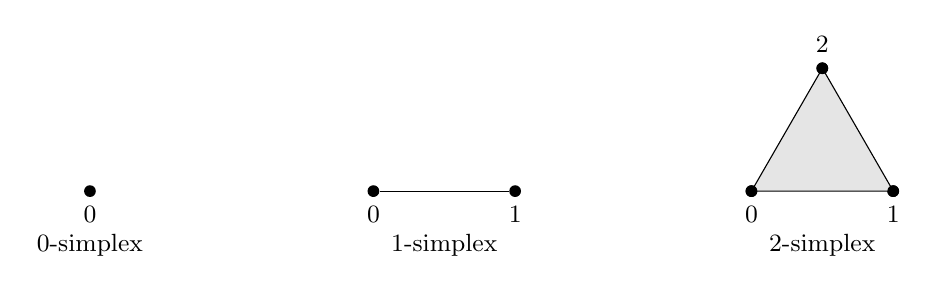
\begin{tikzpicture}[scale=1.2, every node/.style={font=\small}]

% ---- 0-simplex ----
\node[circle, fill=black, inner sep=1.5pt] (v0) at (0,0) {};
\node[below=2pt] at (v0) {$0$};
\node[below=12pt] at (0,0) {0-simplex};

% ---- 1-simplex ----
\node[circle, fill=black, inner sep=1.5pt] (v1a) at (3,0) {};
\node[circle, fill=black, inner sep=1.5pt] (v1b) at (4.5,0) {};

\draw (v1a) -- (v1b);

\node[below=2pt] at (v1a) {$0$};
\node[below=2pt] at (v1b) {$1$};

\node[below=12pt] at (3.75,0) {1-simplex};

% ---- 2-simplex ----
\node[circle, fill=black, inner sep=1.5pt] (v2a) at (7,0) {};
\node[circle, fill=black, inner sep=1.5pt] (v2b) at (8.5,0) {};
\node[circle, fill=black, inner sep=1.5pt] (v2c) at (7.75,1.3) {};

% \filldraw[fill=gray!20, draw=black] 
%   (v2a.center) -- (v2b.center) -- (v2c.center) -- cycle;
\draw[fill=gray!20] (v2a.center) -- (v2b.center) -- (v2c.center) -- cycle;

\node[circle, fill=black, inner sep=1.5pt] at (v2a.center) {};
\node[circle, fill=black, inner sep=1.5pt] at (v2b.center) {};
\node[circle, fill=black, inner sep=1.5pt] at (v2c.center) {};

\node[below=2pt] at (v2a) {$0$};
\node[below=2pt] at (v2b) {$1$};
\node[above=2pt] at (v2c) {$2$};

\node[below=12pt] at (7.75,0) {2-simplex};

\end{tikzpicture}
$$

Another important class of simplicial sets are horns, which can be thought of as simplices with one face missing.

\begin{definition}[Horn \cite{lurie}]
	For each $n \geq 1$ and $0 \leq i \leq n$, the \emph{$i$-th horn}, denoted as $\L^n_i$, is the simplicial defined as
	\begin{enumerate}
		\item $\L^n_i([m]) = \{f \in \H_{\D}([m], [n]) : [n] \smallsetminus \{i\} \not\subseteq f([m])\}$. 
			In other words, $\L^n_i ([m])$ is the set of all order-preserving maps from $[m]$ to $[n]$ that miss at least one element in $[n] \smallsetminus \{i\}$.
			For the sake of simplicity, we will denote $\L^n_i [m] := \L^n_i ([m])$.
		\item For a map $s \in \H_{\D} ([m], [k])$, the corresponding map $\L^n_i(s): \L^n_i[k] \rightarrow \L^n_i[m]$ are its pullback (see figure below), i.e., for $f \in \L^n_i [k]$ , 
			$$
				\L^n_i(s) (f) = f \circ s
			$$
	\end{enumerate}
	Moreover, $\L^n_i$ is called an \emph{inner horn} if $0 < i < n$, and an \emph{outer horn} if $i = 0$ or $i = n$.
\end{definition}

$$
\begin{tikzpicture}[->, >=Stealth]
  % Nodes
	\node (A) {$[m]$};
	\node[right=of A] (B) {$[k]$};
	\node[below=of B] (C) {$[n]$};

  % Arrows (legs of the right triangle)
  \draw (A) -- node[above] {$s$} (B);
  \draw (B) -- node[right] {$f$} (C);

  \draw[dotted] (A) -- node[below left] {$\L^n_i(f) (k)$} (C);
\end{tikzpicture}
$$

$\L^n_i [m]$ is a functor from $\D\op$ to $\S$ by the standard arguments of pullback.
Because $f \in \L^n_i[k]$, $f$ must miss at least one element in $[n] \smallsetminus \{i\}$, so must $f \circ s$.
Therefore the requirement that $\L^n_i(s) (f) \in \L^n_i [m]$ is satisfied, and the definition is self-consistent.

For each $[m]$, $\L^n_i[m]$ is an subset of $\Delta^n[m]$. Moreover, any $f \in \H_{\D}([m], [k])$, $\Delta^n(f)$ restricts to a map from $\L^n_i[k]$ to $\L^n_i[m]$.
Therefore, we may consider $\L^n_i$ as some kind of a sub-simplicial set of $\Delta^n$.

This intuition is further justified by the geometric realisation of $\L^n_i$, denoted as $|\L^n_i|$, which is $|\Delta^n|$ with the interior and the $i$-th face removed. 
See the following figure for horns contained in the $\Delta^2$.

% Demonstration of horns in 2-simplex
$$
\begin{tikzpicture}[scale=1.2, every node/.style={font=\small}]

% ---- 0-simplex ----
\node[circle, fill=black, inner sep=1.5pt] (v0a) at (0,0) {};
\node[circle, fill=black, inner sep=1.5pt] (v0b) at (1.5,0) {};
\node[circle, fill=black, inner sep=1.5pt] (v0c) at (0.75,1.3) {};
\node[below=2pt] at (v0) {$0$};

\draw (v0b) -- (v0a) -- (v0c);

\node[below=2pt] at (v0a) {$0$};
\node[below=2pt] at (v0b) {$1$};
\node[above=2pt] at (v0c) {$2$};

\node[below=12pt] at (0.75,0) {$|\L^2_0|$};

% ---- 1-simplex ----
\node[circle, fill=black, inner sep=1.5pt] (v1a) at (3.5,0) {};
\node[circle, fill=black, inner sep=1.5pt] (v1b) at (5,0) {};
\node[circle, fill=black, inner sep=1.5pt] (v1c) at (4.25,1.3) {};

\draw (v1a) -- (v1b) -- (v1c);

\node[below=2pt] at (v1a) {$0$};
\node[below=2pt] at (v1b) {$1$};
\node[above=2pt] at (v1c) {$2$};

\node[below=12pt] at (4.25,0) {$|\L^2_1|$};

% ---- 2-simplex ----
\node[circle, fill=black, inner sep=1.5pt] (v2a) at (7,0) {};
\node[circle, fill=black, inner sep=1.5pt] (v2b) at (8.5,0) {};
\node[circle, fill=black, inner sep=1.5pt] (v2c) at (7.75,1.3) {};

% \filldraw[fill=gray!20, draw=black] 
\draw (v2a.center) -- (v2c.center) -- (v2b.center);

\node[below=2pt] at (v2a) {$0$};
\node[below=2pt] at (v2b) {$1$};
\node[above=2pt] at (v2c) {$2$};

\node[below=12pt] at (7.75,0) {$|\L^2_2|$};

\end{tikzpicture}
$$
